\section{Trabajo práctico integrador Nº 2}

Dado el siguiente ejemplo de estructura organizativa de T.I., Data Center, áreas relacionadas y áreas de control, se solicita:

\begin{figure}[h]
  \centering
  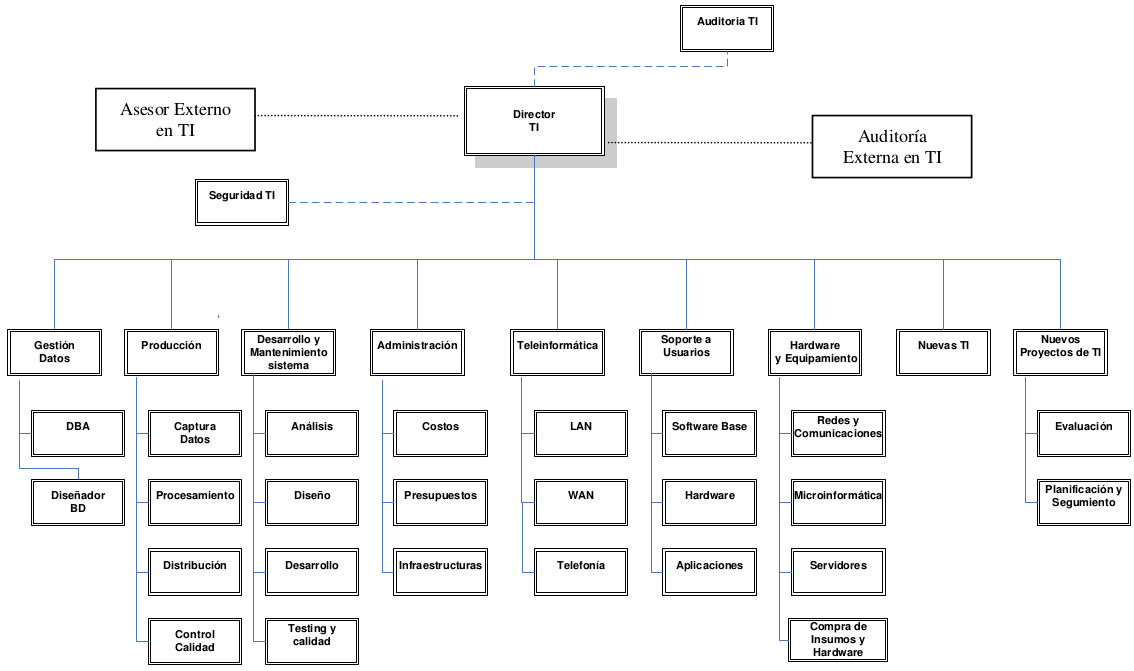
\includegraphics[width=.85\textwidth]{img/tp2_integrador/organigrama}
  \caption{Estructura organizativa de T.I.}
  \label{organigrama-enunciado}
\end{figure}

Para las siguientes \textbf{áreas}:

\begin{itemize}
    \item Área de Producción.
    \item Área de Auditoría externa de T.I.
\end{itemize}


\newpage

	\subsection{Servicios brindados por cada área asignada}
    
    \subsubsection{Servicios del área de Producción}
    
    Principalmente brinda el servicio de definir, desarrollar y gestionar el soporte técnico y funcionamiento de los sistemas de la empresa. 
    Podemos detallar los servicios del área según las actividades que se llevan a cabo:
    
    \begin{comment}
    Esto suena a que es de otras áreas
    \begin{itemize}
		\item Operaciones: Garantizar y fomentar el funcionamiento de la arquitectura de hardware, redes y comunicaciones, operación y sustento de los sistemas de información.
        \item Desarrollo: Aseguramiento de unidades de software con base en los estándares de calidad establecidos, cumpliendo con las especificaciones y requerimientos del mercado.
        \item Arquitectura: Modelar procesos de negocio.
	\end{itemize}
    \end{comment}
    
    \begin{itemize}
		\item Coordinar e implementar todos los procesos, actividades y funciones necesarias para la prestación de los servicios acordados con los niveles de calidad aprobados.
		\item Dar soporte a todos los usuarios de la organización.
		\item Lograr el equilibrio entre estabilidad y capacidad de respuesta.
		\item Proponer mejoras para todos los procesos y actividades involucrados en la gestión y prestación de los servicios TI.
		\item Proponer mejoras que aumenten el ROI (\textit{return of investment} - retorno de la inversión) y VOI (\textit{value on investment} - valor sobre inversión) asociados a los servicios TI.
        \item Coordinar migración de datos entre diferentes sistemas.
        \item Sanear datos recibidos de su formato original a uno compatible con los sistemas.
        \item Ingresar datos provenientes de distintas vías de ingreso.
        \item Servir de soporte a la toma de decisiones estratégicas.
        \item Planear e implementar la distribución de la información procesada del sistema, datos históricos, datos detallados.
        \item Definir los controles que se llevarán a cabo y el procedimiento para realizarlos.
        
	\end{itemize}
    
    \subsubsection{Servicios del área de Auditoría externa de TI}
    
    En primer lugar, una auditoría es una actividad de control, y el hecho de que sea externa quiere decir que es realizada por expertos ajenos a la organización auditada.
    El auditor recoge, agrupa y evalúa evidencias para determinar si un sistema de información:
    
    \begin{itemize}
		\item Protege el activo empresarial.
        \item Mantiene la integridad de los datos.
        \item Lleva a cabo eficazmente los fines de la organización. En caso de que no lo haga, establece los cambios que se deberían realizar para lograr los mismos.
        \item Utiliza eficientemente los recursos.
        \item Cumple con las leyes y regulaciones establecidas.
	\end{itemize}
    
    Por otro lado, analiza el uso de recursos y flujos de información para determinar aquella que es crítica para el cumplimiento de su misión y objetivos, identificando necesidades, duplicidades, costes, valor y barreras, que obstaculizan flujos de información eficientes.
    
    
    \newpage
    
    \subsection{Recomendaciones técnicas y de seguridad física para el Data Center}
    
    \subsubsection{Introducción}
    % http://orbitum.frm.utn.edu.ar/Datacenters/wp-content/uploads/2013/05/1167828372.Norma_ANSI_EIA_TIA_942.pdf
    Se denomina centro de procesamiento de datos (CPD), o \textit{data center}, a aquella ubicación donde se concentran, de forma adecuada y eficiente, los recursos necesarios para el procesamiento de la información de una organización.
    
    % tambien puedo hablar de normas nacionales e internacionales de construcción como TIA, EIA, NFPA, USGBC, RoHS, ASHRAE, NFPA, ANSI, IRAM, IEC, IEEE, CENELEC, AEA, ICREA, Uptime Institute y BICSI.
    Para definir las características que debe tener un Data Center es necesario determinar para qué se utilizará y la fiabilidad que debe tener. La norma  ANSI/TIA-942 divide a los datacenter en 4 Tiers. El concepto de Tier nos indica el nivel de fiabilidad de un centro de datos. A mayor número en el Tier, mayor disponibilidad, y por lo tanto mayores costes asociados en su construcción y más tiempo para hacerlo. A día de hoy se han definido cuatro Tier diferentes, y ordenados de menor a mayor son:
    
      \begin{itemize}
          \item \textbf{Tier 1: Centro de datos Básico} 
            \begin{itemize}
                \item El servicio puede interrumpirse por actividades planeadas o no planeadas.
                \item No hay componentes redundantes en la distribución eléctrica y de refrigeración.
                \item Puede o no puede tener suelos elevados, generadores auxiliares o UPS.
                \item Tiempo medio de implementación, 3 meses.
                \item La infraestructura del \textit{data center} deberá estar fuera de servicio al menos una vez al año por razones de mantenimiento y/o reparaciones.
                \item Disponibilidad del \textbf{99.671\%}.
            \end{itemize}

          \item \textbf{Tier 2: Centro de datos Redundante}
            \begin{itemize}
                \item  Menos susceptible a interrupciones por actividades planeadas o no planeadas.
                \item  Componentes redundantes (\textit{N+1})
                \item  Tiene suelos elevados, generadores auxiliares o UPS.
                \item  Conectados a una única línea de distribución eléctrica y de refrigeración.
                \item  De 3 a 6 meses para implementar.
                \item  El mantenimiento de esta línea de distribución o de otras partes de la infraestructura requiere una interrupción de las servicio.
                \item Disponibilidad del \textbf{99.741\%}.
            \end{itemize}


          \item  \textbf{Tier 3: Centro de datos Concurrentemente Mantenibles}
            \begin{itemize}
                \item Permite planificar actividades de mantenimiento sin afectar al servicio de computación, pero eventos no planeados pueden causar paradas no planificadas.
                \item  Componentes redundantes (N+1)
                \item Conectados  múltiples líneas de distribución eléctrica y de refrigeración, pero únicamente con una activa.
                \item De 15 a 20 meses para implementar.
                \item Hay suficiente capacidad y distribución para poder llevar a cabo tareas de mantenimiento en una línea mientras se da servicio por otras.
                \item Disponibilidad del \textbf{99.982\%}.
            \end{itemize}


          \item  \textbf{Tier 4: Centro de datos Tolerante a fallos} 
            \begin{itemize}
                \item  Permite planificar actividades de mantenimiento sin afectar al servicio de computación críticos, y es capaz de soportar por lo menos un evento no planificado del tipo ``peor escenario'' sin impacto crítico en la carga.
                \item  Conectados múltiples líneas de distribución eléctrica y de refrigeración con múltiples componentes redundantes (2 (N+1) significa 2 UPS con redundancia N+1).
                \item  De 15 a 20 meses para implementar.
                \item Disponibilidad del \textbf{99.995\%}.
            \end{itemize}

      \end{itemize}

    %http://www.gzingenieria.com/pdf/ConfCarlosZuluagaMar8.pdf
    %http://blog.aodbc.es/2012/07/10/clasificacion-tier-en-el-datacenter-el-estandar-ansitia-942/
    %http://www.c3comunicaciones.es/data-center-el-estandar-tia-942/
  Lo anteriormente expuesto nos brinda un panorama general que nos permitirá elegir las características que debe tener el Data Center, permitiendo de este modo equilibrar la inversión y la fiabilidad.
  
  %http://www.creacionempresas.com/index.php/plan-de-viabilidad/que-es-un-plan-de-empresa-viabilidad/produccion-y-operaciones
  %http://www.datacenterdynamics.es/focus/archive/2012/03/diez-aspectos-fundamentales-tener-en-cuenta-para-construir-un-datacenter
  Las empresas IT hacen gran uso de los servidores es por esto que se utilizará un data center de \textbf{\textit{Tier} 3}, o con características similares, ya que pretendemos un alto nivel de redundancia y un nivel de inactividad lo más bajo posible que se pueda implementar a un costo razonable.
  Este último motivo es el que nos lleva a no elegir un \textit{Tier} de nivel 4.
  A continuación se detallan las recomendaciones a seguir:
 

 
  \subsubsection{Recomendaciones técnicas}
  
    \begin{itemize}
        \item \textbf{Ubicación lógica: } La ubicación lógica  viene determinada por quién tiene acceso a los datos. En nuestra caso será la empresa de IT ubicada en Mendoza quien accederá a los servidores de producción y calidad.
        \item \textbf{Ubicación física:} Alejado de zonas con humedad, de zonas en las que transiten vehículos de carga pesada (ya que las vibraciones afectan a los servidores.) y alejado de zona de acceso de personal no autorizado, no se recomienda que esté en un subsuelo cerca de instalaciones de agua. El lugar recomendado para un data center es ente los pisos del medio de un edificio.
        \item Prever la construcción de un data center secundario a una cierta distancia del principal. Para zonas sismícas recomendables 5km de distancia y en zonas no sísmicas 2.5 km.
        \item \textbf{Espacio y diagrama de distribución:} El inmueble es muy costoso, por lo tanto debe asegurarse de que haya suficiente espacio y que se use prudentemente, para ello se considera una posible expansión a futuro. A continuación se detallan las áreas que poseerá el data center:
        \begin{itemize}
            \item Un cuarto de entrada: este cuarto posee los equipos de los operadores de telefonía, y se encontrará ubicado afuera del data center por razones de seguridad.
            \item Un área de distribución principal: Alberga el punto de conexión cruzada central para el sistema de cableado estructurado del área de producción. Se recomienda racks separados para los cables de fibra, UTP y coaxial.
            \item Un área de distribución horizontal: Es la ubicación de la interconexión horizontales, es el punto de distribución para el cableado hacia las áreas de distribución de los equipos. Se recomienda un máximo de 2000 cables UTP de 4 pares o terminaciones coaxiles.
            \item Un área de distribución de zona: Es el área de cableado estructurado para los equipos que van en el suelo no puede aceptar paneles de patcheo.
            \item Un área de distribución de equipos: Aquí se encuentran ubicados los gabinetes y racks de equipos. La norma especifica que los gabinetes y racks se deben colocar en una configuración ``hot aisle/cold aisle'' para que disipen de manera eficaz el calor de los equipos electrónicos.
        \end{itemize}
        \item Instalación de falsos suelos y falsos techos. Los falsos suelos deben soportar el peso de los equipos que serán instalados.
        \item \textbf{Administración de cables}:
            \begin{itemize}
                    \item Se recomienda usar racks comunes en toda la distribución principal y las áreas de distribución horizontal para simplificar el montaje del rack y brindar un control unificado de los cables.
                    \item Se recomienda instalar administradores de cables vertical y horizontal, comunes y extensos dentro de y entre los racks para garantizar una administración de cables eficaz y prever un crecimiento ordenado.
                    \item Se recomienda instalar extensas trayectorias de cables (por arriba y por debajo del piso), para garantizar una administración de cables eficaz y prever un crecimiento ordenado.
                    \item Se recomienda separa los cables UTP y coaxiales de la fibra óptica en las trayectorias horizontales para evitar aplastarla. Los cables eléctricos van en bandeja de cables y la fibra, en canales montados en bandejas.
                    \item El tendido de fibra debe hacerse en un sistema de canales para evitar que se dañe.
            \end{itemize}
         \item  \textbf{Energía}:
            \begin{itemize}
	            \item Se recomienda tener dos o más alimentaciones de energía de la empresa de servicio.
                \item Doble acometida eléctrica.
                \item Muelle de carga y descarga.
                \item Suministro de alimentación ininterrumpible (UPS, por sus reglas en inglés:Uninterrupted power supplies )
                \item Circuitos múltiples para los sistemas de computo y comunicaciones y para equipos de enfriamiento
            \end{itemize}
          \item \textbf{Refrigeración}:           
          \begin{itemize}
          \item Se recomiendan equipos de refrigeración adecuados
          \item Buena circulación de aire, se recomienda un procedimiento conocido como ``hot aisle/cold aisle''. En una configuración hot aisle/cold aisle, los racks de los equipos se disponen en filas alternas de pasillos calientes y fríos. En el pasillo frío, los racks de los equipos se disponen frente a frente. 
En el pasillo caliente, están dorso contra dorso. Las placas perforadas en el piso elevado de los pasillos fríos permiten que llegue aire frío al frente de los equipos. Este aire frío envuelve al equipo y se expulsa por la parte trasera hacia pasillo caliente. En el pasillo caliente, desde luego, no hay placas perforadas para evitar que se mezclen el aire caliente con el frío. Para obtener los mejores resultados con este método, los pasillos deben tener dos azulejos de ancho para permitir el uso de placas perforadas en ambas filas, si fuera necesario.
	      \item Aumentar la altura del piso elevado. Duplicar la altura del piso ha demostrado aumentar la corriente de aire hasta un 50\%.
          \item Usar racks abiertos en lugar de gabinetes. Si no se puede usar racks por motivos de seguridad o por la profundidad de los servidores, se puede usar gabinetes con una malla en el frente y el dorso como alternativa.
          \item Aumentar la corriente de aire debajo del piso al bloquear todos los escapes de aire innecesarios.
          \item Reemplazar las placas perforadas actuales con otros con agujeros más grandes. La mayoría de las placas vienen con 25\% de agujeros, pero algunos tienen entre 40 y 60\% de agujeros.
          \end{itemize}
          \item Por último es recomendable la creación de zonas desmitarizadas (DMZ), realizar segmentación de redes locales y crear redes virtuales (VLAN).
    \end{itemize}
  
  
  \subsubsection{Recomendaciones de seguridad física}
  Las principales amenazas que se prevén en la seguridad física son:
      \begin{itemize}
          \item     Desastres naturales, incendios accidentales tormentas e inundaciones.
          \item   Amenazas ocasionadas por el hombre.
          \item    Disturbios, sabotajes internos y externos deliberados.
      \end{itemize}
Para evitarlas a continuación se listan las siguientes recomendaciones:

      \begin{itemize}
	      \item 
          \item \textbf{Salidas de emergencia:} Estas deben estar liberadas y bien iluminadas, se recomienda que la puerta de acceso posea un ancho de 95cm y que abra hacia afuera.
          \item \textbf{Medidas de seguridad en caso de incendio o inundación:} drenajes, extintores, vías de evacuación, puertas ignífugas, etc.
          \item Instalar sistemas de detección y extinción de incendios.
          \item Se recomienda utilizar materiales de construcción no combustibles y resistentes la fuego.
          \item Recubrir las paredes con pintura lavable, con el objeto de que no se desprenda polvo y sea fácil su limpieza.
		  \item Construir el mínimo de ventanas exteriores (o ninguna) a fin de evitar interferencias. 
          \item Instalar alarmas, controles de temperatura y humedad con avisos SNMP o SMTP.
          \item Poseer cerraduras electromagnéticas, torniquetes.
		  \item Es recomendable instalar cámaras de seguridad y detectores de movimiento.
	      \item Es recomendable utilizar tarjetas de identificación, para el control de acceso a salas.
          \item Definir un control de acceso a nivel de racks.
          \item Es recomendable establecer cuales serán las salas y las cajas de backup.
          \item Es recomendable que el data center posea aislación sonora y térmica.
          \item Asegurar que tareas de contingencias ante la ocurrencia de alguno de los riesgos definidos puedan realizarse de forma automática y manual. Por ejemplo el apagado de un equipo, alcanzada cierta temperatura, debe estar previsto de manera automática pero también debe existir un mecanismo de apagado manual por si los mecanismos de apagado manual fallen.
          \item Las llaves del lugar deben estar en un lugar seguro y se debe registrar la gente que entra al lugar

          
      \end{itemize}
  
  

  
\newpage

\subsection{Aplicación de ``Retroalimentación a 360''} % en las áreas asignadas.

\subsubsection{Introducción}


\paragraph{Concepto}

La \textbf{evaluación de retroalimentación de 360 grados} (también conocida como \textit{``evaluación integral''} es un método que incluye reactivos de evaluación de múltiples niveles dentro de la empresa, así como de fuentes externas.
Se lama así debido a que considera todas las relaciones representativas que tiene el evaluado a su alrededor.

En este método, todas las personas que se relacionan con el empleado evaluado, como directivos, el empleado mismo, supervisores, subordinados, colegas, miembros del equipo, así como clientes internos o externos, le asignan una calificación.

A diferencia de los enfoques tradicionales, la retroalimentación de 360 grados se centra en las habilidades necesarias a través de los límites organizacionales.
Además, al compartir la responsabilidad de la evaluación entre varias personas, muchos de los errores comunes de la evaluación se pueden reducir o eliminar.
El método de retroalimentación de 360 grados proporciona una medida más objetiva del desempeño de una persona.
La inclusión de la perspectiva de múltiples fuentes da como resultado un punto de vista más amplio del desempeño del empleado y minimiza tendencias que surgen de puntos de vista limitados del comportamiento.


\paragraph{Utilidad}

Los principales usos que se da a la retroalimentación de 360 grados son las siguientes:

\begin{itemize}
    \item Medir el desempeño del personal.
    \item Medir las competencias.
    \item Diseñar programas de desarrollo.
\end{itemize}

Esta herramienta pretende dar a los trabajadores de la compañía, y a su compañía, una perspectiva de su desempeño lo más adecuada posible, al obtener \textit{inputs} desde todos los ángulos: Jefes, compañeros, subordinados, clientes internos, clientes externos, entre otros.

El propósito de aplicar la evaluación de retroalimentación de 360 grados es darle al profesional la retroalimentación necesaria para tomar las medidas para mejorar su desempeño, su comportamiento, o ambos, y dar a la dirección de la empresa la información necesaria para tomar decisiones en el futuro.


\paragraph{Objetivos}

Los objetivos de realizar una evaluación de retroalimentación de 360 grados son:

\begin{itemize}
    \item Conocer el desempeño de cada uno de los evaluados de acuerdo a diferentes competencias requeridas por la organización y el puesto en particular.
    \item Detectar áreas de oportunidad del individuo, del equipo y de la organización.
    \item Llevar a cabo acciones precisas para mejorar el desempeño del personal y, por lo  tanto, de la organización.
\end{itemize}

El verdadero objetivo de las evaluaciones de retroalimentación de 360 grados es el \textbf{desarrollo de las personas}.
El desarrollo personal, que es esencial en el lugar de trabajo, requiere una retroalimentación adecuada, honesta, planteada y específica.

La evaluación de retroalimentación de 360 grados será una buena herramienta para el desarrollo de competencias del personal, siempre que se haya diseñado con base a los comportamientos esperados para la organización en particular.
De ese modo serán los comportamientos necesarios para alcanzar los objetivos deseados.


\subsubsection{Método de evaluación}

Para las diferentes áreas, la persona a evaluar será el \textbf{gerente} de la misma, y se tendrá en cuenta la calificación que realizarán los distintos evaluadores sobre aspectos determinados.
Una vez realizada la evaluación, y considerando la ponderación asignada a cada tipo de evaluador, se obtendrá una calificación promedio de cada aspecto.
Es importante, para aplicar efectivamente este método de evaluación, garantizar la confidencialidad de todos los evaluadores participantes.

En el \textbf{Cuadro \ref{evaluadores-ponderacion}} se explicitan los diferentes tipos de evaluadores, su descripción y la ponderación asignada por los mismos en la evaluación.

\begin{table}[h]
    \centering
    \resizebox{\textwidth}{!}{
        \begin{tabular}{|l|l|l|}
            \hline
            \multicolumn{1}{|c|}{\textbf{Tipo de evaluador}} & \multicolumn{1}{c|}{\textbf{Descripción}} & \multicolumn{1}{c|}{\textbf{Ponderación}} \\ \hline
            \textbf{Superior jerárquico} & Persona que se ubica por encima del evaluado, en la estructura jerárquica. & \textbf{0,20} \\ \hline
            \textbf{Colegas} & Personas ubicadas en el mismo nivel jerárquico que el evaluado, poseen responsabilidades laborales y experiencia similares. & \textbf{0,15} \\ \hline
            \textbf{Subordinados} & Personas a cargo del evaluado, ubicados directamente por debajo en la estructura jerárquica. & \textbf{0,15} \\ \hline
            \textbf{Clientes internos} & Compañeros de la organización, que están relacionados en forma directa o indirecta con las actividades desarrolladas por el evaluado. & \textbf{0,20} \\ \hline
            \textbf{Clientes externos} & Personas ajenas a la organización, que están relacionadas con las actividades desarrolladas por el evaluado. & \textbf{0,30} \\ \hline
        \end{tabular}
    }
    \caption{Descripción y ponderación de los diferentes evaluadores.}
    \label{evaluadores-ponderacion}
\end{table}

Una vez realizadas las calificaciones de cada aspecto por los distintos evaluadores, se completa una planilla para obtener un promedio por aspecto y un promedio general.
De esta manera, se podrá identificar las características a mejorar y, al mismo tiempo, obtener una calificación general sobre el desempeño del área.

En el \textbf{Cuadro \ref{evaluacion-retroalimentacion}} se aprecia el formato de la tabla de evaluación, que contiene la totalidad de los evaluadores en las columnas, los aspectos a evaluar en las diferentes filas, y la columna final que especifica el promedio de cada aspecto relevado, y el promedio general de la evaluación.  

\begin{table}[h]
    \centering
    \resizebox{\textwidth}{!}{%
        \begin{tabular}{|c|c|c|c|c|c|c|}
            \hline
            \textbf{} & \textbf{Superior jerárquico} & \textbf{Colegas} & \textbf{Subordinados} & \textbf{\begin{tabular}[c]{@{}c@{}}Clientes\\ internos\end{tabular}} & \textbf{\begin{tabular}[c]{@{}c@{}}Clientes\\ externos\end{tabular}} & \textbf{Promedio} \\ \hline
            \textbf{Aspecto 1} &  &  &  &  &  &  \\ \hline
            \textbf{Aspecto 2} &  &  &  &  &  &  \\ \hline
            \textbf{...} &  &  &  &  &  &  \\ \hline
            \textbf{Aspecto N} &  &  &  &  &  &  \\ \hline
            \multicolumn{6}{|r|}{\textbf{Promedio general}} & \multicolumn{1}{l|}{} \\ \hline
        \end{tabular}
    }
    \caption{Tabla de evaluación de retroalimentación de 360 grados.}
    \label{evaluacion-retroalimentacion}
\end{table}


\subsubsection{Retroalimentación de 360 grados en el área de Producción}

Los evaluadores existentes, encargados de calificar la labor y desempeño del \textbf{Gerente de Producción}, se muestran en el \textbf{Cuadro \ref{evaluadores-produccion}}.


\begin{table}[h]
    \centering
    \resizebox{\textwidth}{!}{%
        \begin{tabular}{|l|l|}
            \hline
            \multicolumn{1}{|c|}{\textbf{Tipo de evaluador}} & \multicolumn{1}{c|}{\textbf{Cargo}} \\ \hline
            \textbf{Superior jerárquico} & Director de TI. \\ \hline
            \textbf{Colegas} &
                \begin{tabular}[c]{@{}l@{}}
                    Gerente de Gestión de datos. \\
                    Gerente de Desarrollo y mantenimiento de sistemas. \\
                    Gerente de Administración. \\
                    Gerente de Teleinformática. \\
                    Gerente de Soporte a usuarios. \\
                    Gerente de Nuevas TI.
                    Gerente de Nuevos proyectos de TI.
                \end{tabular} \\ \hline
            \textbf{Subordinados} &
                \begin{tabular}[c]{@{}l@{}}
                    Jefe de Captura de datos. \\
                    Jefe de Procesamiento. \\
                    Jefe de Distribución. \\
                    Jefe de Control de calidad.
                \end{tabular} \\ \hline
            \textbf{Clientes} &
                \begin{tabular}[c]{@{}l@{}}
                    \textbf{Externos}: Clientes y proveedores de la organización, ajenos a la misma. \\
                    \textbf{Internos}: Usuarios de los sistemas propios de la organización.
                \end{tabular} \\ \hline
        \end{tabular}
    }
    \caption{Evaluadores del Gerente de Producción.}
    \label{evaluadores-produccion}
\end{table}

Los aspectos a evaluar, concernientes directamente al desempeño y rendimiento del \textbf{Gerente de Producción}, son los siguientes:

\begin{itemize}
    \item Comunicación.
    \item Resolución de problemas.
    \item Delegación de tareas.
    \item Iniciativa.
    \item Trabajo en equipo.
    \item Motivación.
    \item Compromiso.
\end{itemize}


\subsubsection{Retroalimentación de 360 grados en el área de Auditoría externa de TI}

Los evaluadores existentes, encargados de calificar la labor y desempeño del \textbf{Auditor externo}, se muestran en el \textbf{Cuadro \ref{evaluadores-auditoria-externa}}.


\begin{table}[h]
    \centering
    \resizebox{\textwidth}{!}{%
        \begin{tabular}{|l|l|}
            \hline
            \multicolumn{1}{|c|}{\textbf{Tipo de evaluador}} & \multicolumn{1}{c|}{\textbf{Cargo}} \\ \hline
            \textbf{Superior jerárquico} & No cuenta con superior jerárquico. \\ \hline
            \textbf{Colegas} &
                \begin{tabular}[c]{@{}l@{}}
                    Director de TI. \\
                    Auditor de TI. \\
                    Asesor externo en TI.
                \end{tabular} \\ \hline
            \textbf{Subordinados indirectos} &
                \begin{tabular}[c]{@{}l@{}}
                    Gerente de Gestión de datos. \\
                    Gerente de Desarrollo y mantenimiento de sistemas. \\
                    Gerente de Administración. \\
                    Gerente de Teleinformática. \\
                    Gerente de Soporte a usuarios. \\
                    Gerente de Nuevas TI. \\
                    Gerente de Nuevos proyectos de TI.
                \end{tabular} \\ \hline
            \textbf{Clientes internos} & Empleados de la organización. \\ \hline
        \end{tabular}
    }
    \caption{Evaluadores del Auditor externo de TI.}
    \label{evaluadores-auditoria-externa}
\end{table}

Los aspectos a evaluar, concernientes directamente al desempeño y rendimiento del \textbf{Auditor externo de TI}, son los siguientes:

\begin{itemize}
    \item Comunicación.
    \item Orientación y establecimiento de lineamientos para la organización.
    \item Compromiso.
    \item Relevancia de las observaciones.
    \item Nivel de capacitación.
\end{itemize}




%http://www.jovitae.com/blog/?p=123

\newpage

    \subsection{Aplicación del ``Coaching Eficaz''} %en las áreas asignadas.
        %http://sg.com.mx/revista/42/coaching-y-produccion
        \subsubsection{Coaching en el área de Producción}
		 Para que el desempeño de los empleados sea el óptimo en necesario profundizar la interacción personal-gerente que permita entrar en un clima de confianza y lograr de este modo potenciar las características del personal que harán que el área de producción mejore sustancialmente. Para esto es necesario que el Coach sepa:
        \begin{itemize}
            \item Escuchar
            \item Acompañar
            \item proveer
            \item motivar
        \end{itemize}
Las técnicas que se utilizan para este fin son variadas y aplicadas directamente por el interesado, donde un programa preestablecido entre el coach y el coaching   o alumno determinan los tiempos y eventos, así como los criterios para calificar el desarrollo. 

\paragraph{Beneficios de aplicar coaching}

\textbf{Personales}:

      \begin{itemize}
      \item Equilibrio en la vida laboral, familiar y personal.
      \item Abandono de la rutina.
      \item Desarrollo de habilidades para adaptarse rápidamente al cambio
      \item Mejora e aprendizaje.
      \item manejo del estrés, ansiedad y elementos distractores.
      \item Aumentar su autoestima y confianza en sí mismo.
      \item Superar tus bloques y obstáculos.
      \end{itemize}
      
\textbf{Interpersonales}:
\begin{itemize}
\item Comunicación eficaz.
\item mayor actitud para negociación.
\item Adaptación al cambio
\item Formación y trabajo en equipo.
\item Aprendizaje continúo.
\end{itemize}

Las actividades a realizar para ejercer el coaching en el área de producción son:
\begin{itemize}
\item Reuniones diarias cortas para definir las actividades a realizar en el día.
\item Reuniones semanales, donde:
    \begin{itemize}
    \item Se inicien discusiones que incentiven al personal a ofrecer ideas.
    \item Permita descubrir cuales son las actividades en las que la persona se siente más cómoda para determinar que actividad asignarle.
    \item felicitar por los resultados y reencaminar cuando hay fracasos
	\item consultar sobre objetivos y proyectos actuales
    \end{itemize}

\item Reuniones mensuales donde el tema fundamental son los sentimientos, emociones y deseos: Estas emociones y problemas guardadas en el inconsciente tienen una gran influencia en las decisiones, como gerentes, es nuestra responsabilidad encontrarlas, presentárselas al individuo y resolverlas. Para lograr un alto nivel de confianza y encontrar estos sentimiento ocultos se van a implementar diversas actividades como:
%http://sg.com.mx/revista/42/coaching-y-produccion
    \begin{itemize}
    \item Ejercicios de relajación.
    \item Yoga con música relajante: ayuda al control de las reacciones y emociones.
	\item Realizar ejercicios de autoconocimiento.
    \end{itemize}
%http://marcaladiferencia.com/las-10-caracteristicas-del-coaching-eficaz/

\item Detectar las situaciones sentimentales de los integrantes del equipo

\item Inspirar con el ejemplo: animar al personal a asumir riesgos y considerar al fracaso como una posibilidad

\item Comunicar correctamente y con claridad las actividades a realizar.
    \begin{itemize}
    \item Definir resultados esperados
    \item Definir el marco de tiempo o el \textit{deadline}.
    \item Definir los recursos disponibles.
    \item Definir como la tarea o proyecto que se alinean con los objetivos de la empresa, o cliente.
    \item Definir que dependencias existen para completar esta tarea o proyecto.
    \item Definir la recompensa en el caso de  lograr el éxito y lo que el éxito significa en este caso.
    \item Indicar el precio del fracaso y las consecuencias a nivel de departamento.
    \end{itemize}
\item Mantener blogs internos o contacto por redes sociales donde el equipo expone y comparte sus ideas y los momentos compartidos para amplificar la cohesión.
\end{itemize}

         
        \subsubsection{Coaching en el área de Auditoría externa de TI}        
        El área de auditoría  suele provocar conflictos internos en la organización ocasionando situaciones incómodas entre los miembros del equipo, por ello es de fundamental importancia promover el respeto entre el personal, educando a los miembros del sector para que sean capaces de transmitir las decisiones sin perjudicar las relaciones laborales.
        %https://nuestrofuturo12061.wordpress.com/el-auditor-informatico/
        %recomendaciones y soluciones que aporte deben estar alineadas a los objetivos de la empresa y a los recursos que se poseen.
        \begin{itemize}
	        \item Las reuniones estarán orientadas a comunicar los objetivos y recursos que posee la empresa.
            \item Se realizarán reuniones mensuales de todo el sector de IT para que el área de auditoría conozca a todos los participantes y de este modo sepa como relacionarse con cada uno de ellos.
            \item Fomentar el reconocimiento de sus capacidades, aptitudes y carencias.
            \item Transmitirle de forma continua a los responsables del área, cuales son las políticas de la empresa y cuáles son los derechos económicos a proteger.
            \item  El coach debe observar el estado sentimental de los participantes del área, y de este modo detectar situaciones que no produzcan los resultados esperados.
            \item El coach debe tener comunicación continua que garantice conocer en profundidad a los miembros del área.
            
        \end{itemize}



\newpage

    \subsection{Características de equipos de trabajo efectivos y equilibrados} %Con ejemplos dentro de sus áreas, e 5:10
    

\subsubsection{Equipo de trabajo efectivo}

Un equipo de trabajo efectivo presenta las siguientes \textbf{características}:

\begin{itemize}
    \item \textbf{Libre expresión} de todos los miembros: Implica que cada miembro del equipo tenga libertad de expresión para poder aportar ideas, y comunicar problemas o limitaciones, al resto del equipo, mejorando así su rendimiento.
    
    \item Principio del \textbf{trabajo en conjunto}, que se logra mediante una delegación eficaz del líder, generando sinergia entre los miembros del equipo de trabajo, cuando los resultados del trabajo en conjunto son mejores que los resultados del trabajo individual.
    
    \item Todos están dispuestos a \textbf{asumir riesgos}, ya que hay una adecuada planificación y gestión de riesgos de parte del líder.
    
    \item Existe \textbf{espíritu de coaching} entre todos los integrantes del equipo, mediante la aplicación de las principales actividades del coaching: Saber escuchar de distintas fuentes y estar atento a lo que le ocurre o piensa cada persona de su equipo, acompañar a cada uno en situaciones difíciles o que no se sabe cómo continuar, proveer los recursos necesarios, contener anímicamente y ayudar en todo lo que fuere necesario para cada persona.

    \item Hay \textbf{objetivos comunes} y \textbf{metas claras} bien arraigados en todos los miembros.
    
    \item Existe iniciativas, deseos y voluntad de \textbf{participación}, \textbf{respeto} por todos y siempre los miembros están dispuestos a colaborar.
    
    \item Aceptación de decisiones por \textbf{consenso general}, aún cuando existan divergencias individuales.
    
    \item \textbf{Buena relación} de los miembros con otros integrantes de otros proyectos y otras áreas, para aprovechar las experiencias ajenas y poner en valor las propias.
    
    \item \textbf{Retroalimentación} de todos los integrantes del equipo de trabajo a los efectos de pensar y poner en práctica permanente acciones de mejora continua.
\end{itemize}


\subsubsection{Equipo de trabajo equilibrado}

Un equipo de trabajo equilibrado presenta las siguientes \textbf{características}:

\begin{itemize}
    \item Cantidad de integrantes, de acuerdo con recomendaciones de alcance de control del líder.
    \item Disponibilidad de tiempo.
    \item Necesidades personales y fines propios.
    \item Actitud (positiva, negativa, colaboración, egoísta, entre otras).
    \item Roles (orientado a la tarea, orientado a la relación, entre otros).
    \item Personalidad (introvertido, extrovertido, agresivo, sumiso, solitario, entre otras).
    \item Ingenio, creatividad, generación de ideas, inquietudes, nuevos proyectos.
    \item Competencias técnicas y nivel de capacitación.
    \item Adaptabilidad al estrés.
\end{itemize}

\subsubsection{Ejemplos de equipos}

\paragraph{Área de Producción}
Para el área de producción un ejemplo de equipo no equilibrado y efectivo es aquel que posee  personal con las mismas características todos con deseos de aportar y brindar distintas soluciones, además en este equipo se realizan continuamente capacitaciones para lograr una excelente nivelación de los conocimientos.
Estás características hacen a que el equipo logre los objetivos pero muchas veces sucede que el exceso de aporte por parte de los integrantes haga que no logren consensuar en una idea provocando que retrasos en la producción.


\paragraph{Área de Auditoría externa de TI}
Un equipo de 2 administradores de bases de datos y 2 encargados de proceso realiza la auditoria de la bas de datos del sistema de una organización "X". Los primeros se encargan del relevamiento, verificación y control de acceso, de actualización y los segundos de controlar la integridad y calidad de los datos obtenidos. Éste presenta un caso de equipo eficaz y equilibrado encargado de auditoría externa.


\newpage

    \subsection{Variables relevantes al contratar personal, en relación a los puestos y perfiles}%Si tuvieran que \textbf{contratar personal} para las áreas asignadas, 10:20 basado en división de puestos y perfiles. seleccionar un puesto
  
    %http://www.intersoftware.org.co/content/conozca-los-cargos-de-las-areas-de-produccion-de-ti
    
    Dado que para cubrir los puestos de las áreas estudiadas se requieren ciertas capacidades o conocimientos técnico, propondríamos que se realicen dos tipo de entrevistas:
    \begin{itemize}
	    \item \textbf{Entrevista técnica}: Para evaluar si el candidato posee las cualidades, fortalezas y habilidades para cubrir ese puesto desde un punto de vista meramente técnico. En este caso se convocará al jefe del sector en cuestión y de ser posible algún usuario clave asociado al proceso. De esta manera aseguramos cubrir la necesidad operativa e involucramos al negocio en el proceso de selección de los individuos de los cuales recibirá soporte.
        \item \textbf{Entrevista de evaluación de habilidades blandas}: Todo postulante que cubra las necesidades técnicas será entrevistado pos segunda vez. En esta ocasión se organizarán entrevistas grupales en donde se planteen situaciones a solucionar, y en las cuales un psicólogo participará como observador, analizando las características de personalidad de cada individuo.
           \end{itemize}


    \subsubsection{Área de Producción}
          \begin{itemize}
          \item Variables generales a tener en cuenta
              \begin{itemize}
                  \item  No realizar tareas de línea 
                  \item Calidad profesional 
                  \item Sólida formación en auditoria 
                  \item Sentido común 
                  \item Sensatez de juicio 
                  \item Espíritu de observación 
                  \item Creatividad 
                  \item Capacidad de análisis lógico 
                   \item Lograr aceptación del auditado por efecto de su capacidad técnica y no como consecuencias de informes o excesos de autoridad 
                   \item Espíritu docente que le permita transmitir sus conocimientos y recomendaciones con criterio constructivo. 
                   	\item     Mantenerse permanentemente actualizado sobre legislación, normas, actividad de la empresa u organismos  ser auditado.
              \end{itemize}
              
           \item \textbf{Tester-QA}
           
        El tester es la persona encargada de especificar, desarrollar y registrar las pruebas según las especificaciones del sistema, documentando los resultados y las fallas que se detecten.
			\begin{itemize}
			    \item \textbf{Funciones y responsabilidades}
            	
                \begin{itemize}
				    \item Detectar la mayor cantidad de fallas antes de que la aplicación salga a producción.
                    \item Participar de todas las etapas del proceso de desarrollo de software, colaborando para asegurar la máxima calidad del producto.
                    \item Revisar las funcionalidades de la aplicación para corroborar su correcto funcionamiento de acuerdo a lo planificado.
				\end{itemize}
            
            \item \textbf{Perfil}
            \begin{itemize}
				\item Capacidad de abstracción y modelado para atender y simular el comportamiento del sistema bajo prueba.
                \item Facilidad de comunicación oral y escrita para interactuar con desarrolladores y usuarios.
                \item Creatividad para generar ideas e imaginar los problemas que podrían existir.
                \item Pensamiento crítico para evaluar las ideas, hacer deducciones y vincular los observado con los criterios de calidad de la empresa.
                \item Aptitudes para el trabajo en equipo, de manera de poder interactuar con los desarrolladores y otros testers, y lograr el máximo beneficio en esta interacción.
            \end{itemize}
            
           \item Procesamiento
           \item Distribución
          \end{itemize}
            \end{itemize}          
            
            
        \subsubsection{Área de Auditoría externa de TI}
            \begin{itemize}
            \item \textbf{Características generales}
                  \begin{itemize}
	                  \item Conocimientos técnicos de las herramientas utilizadas. 
                      \item Perfil analítico y lógico para el análisis de grandes volúmenes de datos. 
                      \item Facilidad para la identificación de patrones que permitan analizar fallos en los procesos ejecutados. 
                      \item  Nivel de motivación personal alta: El tipo de tareas repetitivas a realizar no proveen una motivación extras perfiles más bien inquietos. 
                      \item Facilidad para la confección de informes y comunicación eficaz a los distintos sectores. Forma de evaluar lo solicitado en cada perfil. Test, Entrevistas. 
                  \end{itemize}
           	\item \textbf{Auditor}
            	
                \begin{itemize}
                \item \textbf{Habilidades y destrezas }

                  \begin{itemize}
                      \item Actitud positiva
                       \item Saber escuchar
                       \item Mente analítica
                        \item Capacidad de negociación
                       \item Iniciativa
                       \item Facilidad de trabajaren equipo
                  \end{itemize}
				
                \item \textbf{Características personales}

                    \begin{itemize}
                        \item     Formación y Capacidad Profesional
                        \item    Independencia, Integridad y OBjetividad
                        \item    Diligencia Profesional
                        \item    Responsabilidad
                        \item    Secreto Profesional
                    \end{itemize}


                \end{itemize}
            \end{itemize}   

            
            
            
\newpage
    \subsection{Funciones del Tablero de Comandos, de las áreas asignadas} %11:37
    
    \subsubsection{Área de Producción}
    	\begin{itemize}
			\item\textbf{Tiempo de ejecución de procesos:} se ejecutan procesos automáticos evaluados como críticos para la organización, se contabiliza el tiempo en segundos y se establecen cotas superiores a partir de los cuáles se lanzan las alertas correspondientes.
            \item\textbf{Cantidad de datos procesados:} datos cargados a partir de proceso automatizados ejecutados periódicamente para alimentar el tablero de comando.
            \item\textbf{Tareas planificadas:} notificaciones de tareas previamente programadas y planificadas en el tiempo, backups, actualizaciones de software, renovación de software de seguridad, importación y exportación de datos de un sistema.
            \item\textbf{Tiempo de recuperación luego de fallo:} se controlan los procesos críticos, principalmente su recuperación ante fallos, presentando alertas cuando se superan determinados límites.
            \item \textbf{Carga de procesamiento: }se mide el porcentaje de carga que generan en el servidor los procesos principales.
            \item \textbf{Tickets de soporte cerrados: }promedio de tickets cerrados en función de los elevados.
		\end{itemize}
        
	\begin{figure}[h]
	  \centering
  	  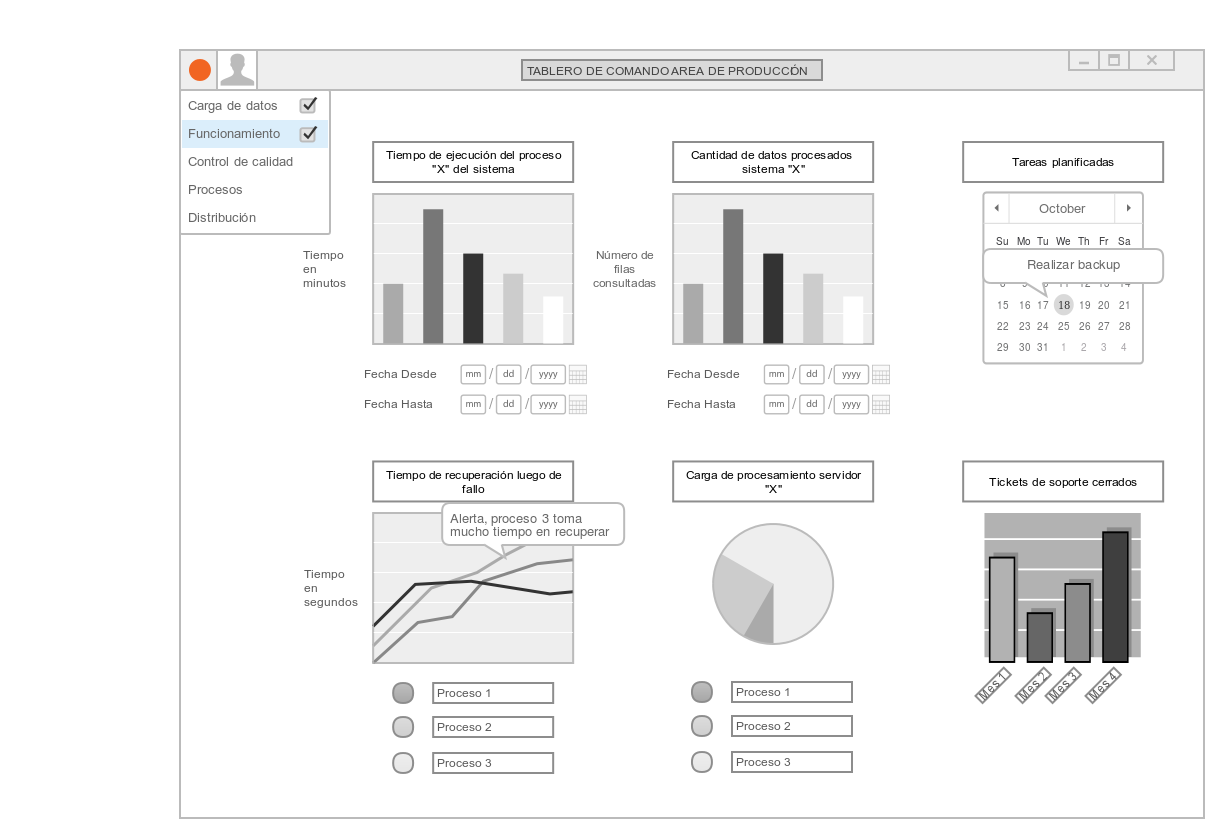
\includegraphics[width=0.85\textwidth]{img/tp2_integrador/area_produccion}
      \label{Área de producción}
      %\caption{}
	\end{figure}
    
    \subsubsection{Área de Auditoría externa de TI}
    	\begin{itemize}
        	\item\textbf{Relación costo beneficio: }detección sistemática de recursos para determinar cuáles son críticos para el cumplimiento de la misión y objetivos.
            \item\textbf{Observaciones: } cantidad de observaciones por sector crítico en el área auditada correspondiente, gestión, legal, datos, bases de datos, seguridad lógica, comunicaciones entre otros. Éstas observaciones nos permite detectar inestabilidades a tiempo para así comunicarlas y poder actuar en consecuencia. Las respuestas a estas detecciones se contabilizan para evaluar el desempeño de la auditoría.
            \item\textbf{Entrevistas: } las entrevistas tanto a auditados como no auditados verifican el grado de confiabilidad del sistema. Verifican asimismo la exactitud, integridad y validez de la información.
			\item\textbf{Satisfacción del usuarios: } determina en que medida el sistema responde a las necesidades del usuario.
            \item\textbf{Recursos: } relación entre recursos planificados y recursos realmente utilizados.
		\end{itemize}    
    
    \begin{figure}[h]
	  \centering
  	  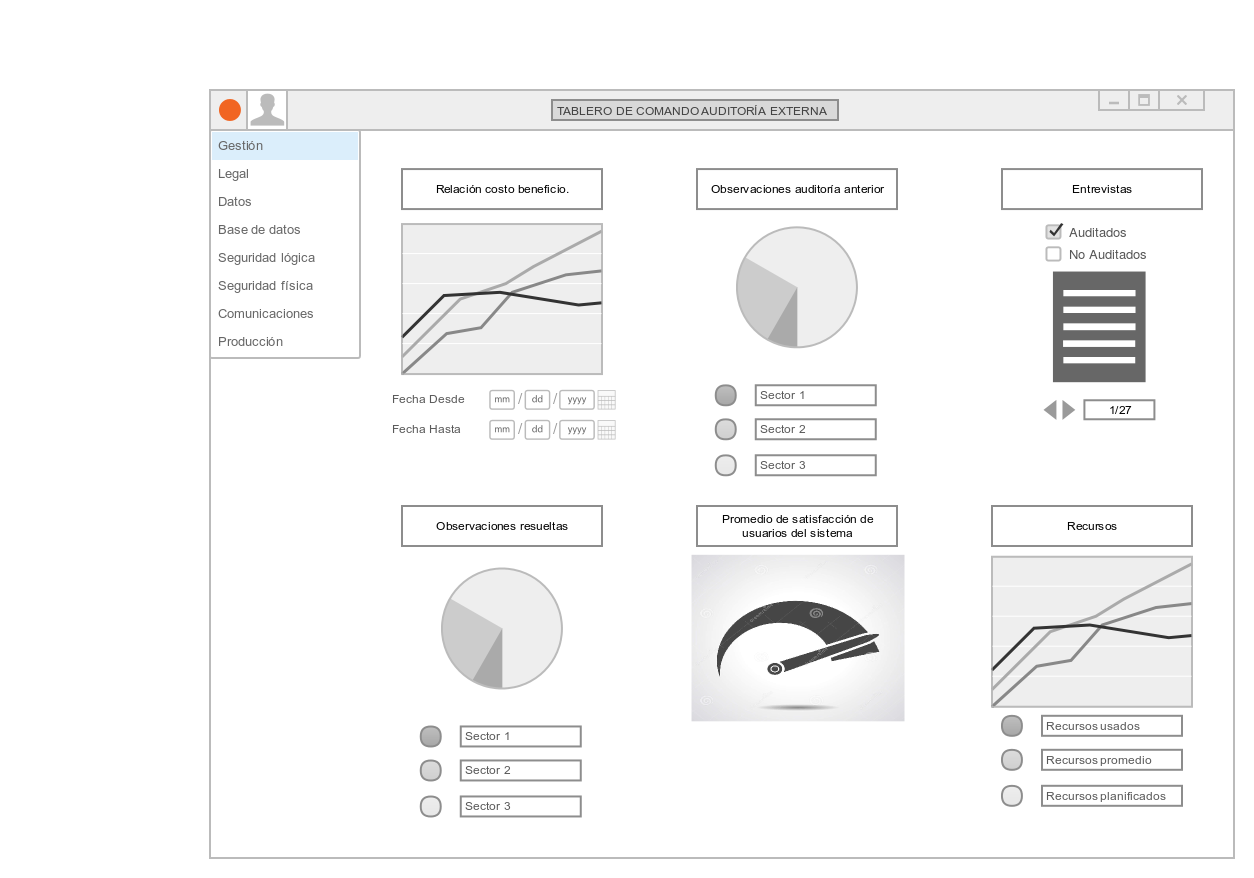
\includegraphics[width=0.85\textwidth]{img/tp2_integrador/auditoria_externa}
      \label{Auditoría externa}
      %\caption{}
	\end{figure}
    
    \subsection{Planificación de estrategia de mejora de las áreas}
    La estrategia tiene que estar orientada a mejorar día a día la calidad en la gestión del área, por ej. mejorar el rendimiento del personal, mejorar los resultados, apoyar a los objetivos de la empresa u organización, tener una adecuada relación con otras áreas,  eficiencia, generación proactiva, reducción de errores, mejoramiento de relaciones interpersonales, satisfacción continua de los Clientes internos y externos, potenciar fortalezas, aprovechar oportunidades, reducir debilidades y estar preparado para las amenazas, 

\begin{center}
\begin{longtable}{|>{\centering\arraybackslash}m{3cm}|>{\centering\arraybackslash}m{3cm}|m{7cm}|}
\caption{Planificación de estrategias de mejora.}
\\

\hline
\textbf{Período}
&
\textbf{Actividad}
&
\multicolumn{1}{c|}{\textbf{Descripción detallada}}
\\
\hline
\endhead
\label{estrategias}
Octubre 2015 a Diciembre 2015
&
Evaluación completa del sector.
&
Se realiza una evaluación de los integrantes del sector (o sólo de cargos superiores, según el presupuesto que se disponga).
Se pretende analizar cómo ven nuestros clientes las tareas ejecutadas por el sector y la respuesta de los integrantes del mismo ante cualquier inquietud.
\\
\hline
Enero 2016 a Febrero 2016
&
Evaluación de procesos y servicios ofrecidos.
&
Se analiza cada proceso, documentándolos para luego poder analizar en detalle su funcionamiento. Se identifican fortalezas y debilidades a resolver.
\\
\hline
Enero 2016 a Febrero 2016
&
Evaluación personal de Recursos Humanos.
&
Se estudia de manera individual a cada integrante de los distintos equipos, en relación con las funciones desarrolladas, cruzando esta información con el estatus relevado de cada proceso.
\\
\hline
Febrero 2016 a Abril 2016
&
Evaluación referente a tecnologías de administración y distribución de datos.
&
Se analiza desde el punto de vista técnico las tecnologías utilizadas, alternativas de implementación y evaluación de costos de la administración y distribución de datos, para finalmente ser presentado a la dirección como parte de la mejora estructural del sector.
\\
\hline
Mayo 2016 a Julio 2016
&
Reestructuración de funciones y optimización del personal.
&
En base al mapeo de procesos y los perfiles de cada uno de los integrantes (con aporte de cada uno ellos), se establecen las posibles tareas para cada uno, priorizando la optimización y eficiencia de los procesos.
\\
\hline
Agosto 2016
&
Revisión y ajuste FODA.
&
Una vez identificadas las fortalezas y debilidades del sector, se  elabora o actualiza la matriz FODA, que también formará parte del análisis de situación actual. La misma permitirá el análisis de las mejoras a implementar, como así también su implementación.
\\
\hline
Julio 2016 a Noviembre 2016
&
Desarrollo de sitio en intranet como soporte a las actividades llevadas a cabo.
&
Como parte de la mejora, se busca publicar de manera efectiva los servicios ofrecidos por el sector, manuales de procesos y herramientas de contacto ante cualquier necesidad del cliente interno.
\\
\hline
Diciembre 2016
&
Relevamiento y publicación de casos de éxito.
&
Se evalúan los casos de éxitos obtenidos hasta el momento y se publica dentro del nuevo sitio. Esto se realiza para alentar a la organización a no generar barreras ante los cambios.
\\
\hline
Enero 2017 a Marzo 2017
&
Capacitación técnica.
&
Como parte de un proceso de mejora de condiciones de los empleados, se ofrece capacitación técnica para aquellos que lo requieran, por especificación de la gerencia o, en su defecto, premiando a aquellos que tengan un buen desempeño y lo soliciten como incentivo.
\\
\hline
Enero 2017 a Marzo 2017
&
Capacitación en Habilidades Blandas.
&
Se capacita a la totalidad del sector en el desarrollo de habilidades blandas y de liderazgo. El objetivo es el desarrollo de un equipo que puede conectarse de manera directa con las necesidades del cliente.
\\
\hline
Abril 2017
&
Confección de SLA (\textit{Service Level Agreements}) y medidas de satisfacción de usuario.
&
Se desarrollan distintas medidas de rendimiento y mecanismos de evaluación por parte del cliente para evaluar el nivel de satisfacción. La información recolectada será utilizada como entrada para la mejora continua del sector.
\\
\hline
Mayo 2017
&
Análisis e implementación de incentivos según evaluación sobre nuevas aptitudes.
&
En base a los resultados obtenidos de las evaluaciones de nuevas aptitudes (obtenidas durante los períodos de capacitación), la evaluación del recurso humano en sí y el visto bueno de la agencia, se implementan incentivos al empleado (remunerativo o no) para premiar el trabajo bien realizado.
\\
\hline
Mayo 2017
&
Publicación de nuevos servicios.
&
Se publican, en el nuevo sitio del sector, los nuevos servicios ofrecidos en base a la evaluación de aptitudes de cada integrante del sector. De esta forma, nos aseguramos poder cubrir cada punto ofrecido a nuestros cliente.
\\
\hline
Junio 2017 a Julio 2017
&
Desarrollo de tablero de comando para el control de SLAs, a nivel de satisfacción y tiempos de respuesta.
&
Se desarrolla un tablero de comando en donde principalmente se muestran los niveles de aceptación de nuestros usuarios, como así también los tiempos de respuesta del sector y la calidad y fiabilidad de la información brindada.
\\
\hline
Julio 2017
&
Evaluación interna entre pares (\textit{peer review}).
&
Se realiza una revisión del trabajo entre pares de un mismo nivel. El mismo sirve como actividad de integración y control entre empleados de la misma jerarquía.
De esta actividad también se desprenden potenciales nuevos lideres.
\\
\hline
Julio 2017
&
Evaluación de posible certificación de procesos internos a través de normas CMMI.
&
En búsqueda de la excelencia del sector, se intenta certificar sobre el estándar de documentación CMMI.
\\
\hline
Agosto 2017
&
Presentación interna de las mejoras obtenidas.
&
Se presenta al equipo las mejoras obtenidas, los esfuerzos realizados y los próximos pasos de mejora (concepto de \textit{mejora continua}).
\\
\hline
Agosto 2017
&
Presentación corporativa de las mejoras introducidas y medidas de rendimiento.
&
Se presenta al directorio los resultados obtenidos y los costos ahorrados en base a las mejoras introducidas. Como incentivo a continuar con el proceso de mejora, se busca más presupuesto en base a los resultados publicados.
\\
\hline
Septiembre 2017
&
Transmisión de conocimiento entre pares.
&
Una vez que el sector se encuentra capacitado por completo, se establece un esquema de transferencia de conocimientos entre pares. En paralelo se desarrolla una matriz de reemplazo que será consultada en caso de ausencia de alguno de los integrantes de los equipos del sector.
\\
\hline
Septiembre 2017
&
Devolución personal a cada empleado del sector.
&
El gerente en persona realiza una devolución personal a cada uno de los integrantes del sector, remarcando los logros individuales como así también los puntos a mejorar. Con esta actividad se busca generar confianza en el equipo con los puestos jerárquicos a los cuales responden.
\\
\hline

\end{longtable}
\end{center}
